%! TeX program = lualatex
\documentclass{beamer}
\usetheme{Madrid}
\usefonttheme[onlymath]{serif}

\usepackage{fontspec}
\setmonofont{DejaVu Sans Mono}[Scale=MatchLowercase]
\newcommand{\verbatimsize}{\footnotesize}

\usepackage{amsmath}

\usepackage{braket}
\usepackage[compat=0.6]{yquant}
\useyquantlanguage{groups}

\title{Quantum Circuits Project}
\author{Ulrik de Muelenaere}
\date{December 15, 2022}

\begin{document}

\begin{frame}
    \titlepage
\end{frame}

\begin{frame}
    \frametitle{Project Goal}
    \begin{itemize}
        \item To write a tool that converts a quantum circuit to a unitary matrix, and vice versa
            \begin{equation*}
                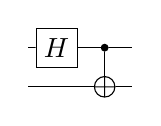
\begin{tikzpicture}[baseline=(current bounding box.center)]
                    \begin{yquant}
                        qubit {} q[2];
                        h q[0];
                        not q[1] | q[0];
                    \end{yquant}
                \end{tikzpicture}
                \quad \Longleftrightarrow \quad
                \frac{1}{\sqrt2} \begin{bmatrix}
                    1 & 1 & 0 & 0 \\
                    0 & 0 & 1 & -1 \\
                    0 & 0 & 1 & 1 \\
                    1 & -1 & 0 & 0
                \end{bmatrix}
            \end{equation*}
        \item Circuit can then be simulated by matrix-vector multiplication
            \begin{equation*}
                \ket{\psi'} = U \ket\psi
            \end{equation*}
    \end{itemize}
\end{frame}

\begin{frame}
    \frametitle{Implementation Overview}
    \begin{itemize}
        \item Implemented in Python using NumPy
        \item \texttt{State} class wraps a complex vector with useful methods
        \item \texttt{Gate} class wraps a unitary matrix with useful methods
        \item \texttt{Circuit} contains a list of \texttt{Gate}s, and is itself a subclass of \texttt{Gate}
        \item \texttt{DecomposedCircuit} is a \texttt{Circuit} consisting of only \textsc{cnot} and single-qubit gates, constructed from an arbitrary unitary matrix
    \end{itemize}
\end{frame}

\begin{frame}[fragile]
    \frametitle{Defining Gates}
    \begin{columns}
        \begin{column}{0.3\textwidth}
            \verbatimsize
\begin{verbatim}
S = Gate(
    name="S",
    num_qubits=1,
    matrix=[
        [1, 0],
        [0, 1j],
    ],
)

Sdagger = S.inverse()

CS = S.control()
\end{verbatim}
        \end{column}
        \begin{column}{0.3\textwidth}
            \begin{align*}
                S & = \begin{bmatrix}
                    1 & 0 \\
                    0 & i
                \end{bmatrix} \\
                S^\dag & = \begin{bmatrix}
                    1 & 0 \\
                    0 & -i
                \end{bmatrix} \\
                CS & = \begin{bmatrix}
                    I & 0 \\
                    0 & S
                \end{bmatrix} \\
                & = \begin{bmatrix}
                    1 & 0 & 0 & 0 \\
                    0 & 1 & 0 & 0 \\
                    0 & 0 & 1 & 0 \\
                    0 & 0 & 0 & i
                \end{bmatrix}
            \end{align*}
        \end{column}
    \end{columns}
\end{frame}

\begin{frame}[fragile]
    \frametitle{Two Ways of Combining Gates}
    \begin{columns}
        \begin{column}{0.3\textwidth}
            \verbatimsize
\begin{verbatim}
A = X @ Y
B = X.tensor_product(Y)
\end{verbatim}
        \end{column}
        \begin{column}{0.3\textwidth}
            \begin{align*}
                A & = X Y \\
                B & = X \otimes Y
            \end{align*}
        \end{column}
        \begin{column}{0.3\textwidth}
            \begin{center}
                \begin{tikzpicture}
                    \begin{yquantgroup}
                        \registers{
                            qubit {} q;
                        }
                        \circuit{
                            box {$A$} q;
                        }
                        \equals
                        \circuit{
                            y q;
                            x q;
                        }
                    \end{yquantgroup}
                \end{tikzpicture}
            \end{center}
            \begin{center}
                \begin{tikzpicture}
                    \begin{yquantgroup}
                        \registers{
                            qubit {} q[2];
                        }
                        \circuit{
                            box {$B$} (q);
                        }
                        \equals
                        \circuit{
                            y q[0];
                            x q[1];
                        }
                    \end{yquantgroup}
                \end{tikzpicture}
            \end{center}
        \end{column}
    \end{columns}
\end{frame}

\begin{frame}[fragile]
    \frametitle{Grover's Algorithm Circuit}
    \begin{columns}
        \begin{column}{0.3\textwidth}
            \verbatimsize
\begin{verbatim}
circuit = Circuit(
    name="Grover",
    num_qubits=3,
)

circuit.add(HHH)

circuit.add(X, [1])
circuit.add(CCZ)
circuit.add(X, [1])

circuit.add(HHH)
circuit.add(XXX)
circuit.add(CCZ)
circuit.add(XXX)
circuit.add(HHH)
\end{verbatim}
        \end{column}
        \begin{column}{0.5\textwidth}
            \begin{center}
                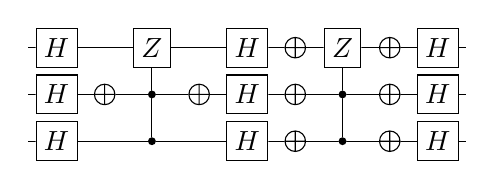
\begin{tikzpicture}
                    \begin{yquant}
                        qubit {} q[3];
                        h q;
                        not q[1];
                        z q[0] | q[1,2];
                        not q[1];
                        h q;
                        not q;
                        z q[0] | q[1,2];
                        not q;
                        h q;
                    \end{yquant}
                \end{tikzpicture}
            \end{center}
        \end{column}
    \end{columns}
\end{frame}

\begin{frame}
    \frametitle{Adding a Gate to a Circuit}
    \begin{itemize}
        \item Consider \texttt{circuit.add(X, [1])} from the previous slide
        \item $X$ must first be padded to a three-qubit gate
            \begin{equation*}
                X' = X \otimes I \otimes I
                \quad \quad \quad
                \begin{tikzpicture}[baseline=(current bounding box.center)]
                    \begin{yquantgroup}
                        \registers{
                            qubit {} q[3];
                        }
                        \circuit{
                            box {$X'$} (q);
                        }
                        \equals
                        \circuit{
                            x q[0];
                            box {$I$} q[1,2];
                        }
                    \end{yquantgroup}
                \end{tikzpicture}
            \end{equation*}
        \item Qubits must be permuted so that $X$ is applied to qubit 1
            \begin{equation*}
                X'' = P^\dag X' P
                \quad \quad \quad
                \begin{tikzpicture}[baseline=(current bounding box.center)]
                    \begin{yquantgroup}
                        \registers{
                            qubit {} q[3];
                        }
                        \circuit{
                            box {$X''$} (q);
                        }
                        \equals
                        \circuit{
                            box {$P$} (q);
                            box {$X'$} (q);
                            box {$P^\dag$} (q);
                        }
                    \end{yquantgroup}
                \end{tikzpicture}
            \end{equation*}
        \item Now the gate matrix can be multiplied with the previous circuit matrix $U$
            \begin{equation*}
                U' = X'' U
                \quad \quad \quad
                \begin{tikzpicture}[baseline=(current bounding box.center)]
                    \begin{yquantgroup}
                        \registers{
                            qubit {} q[3];
                        }
                        \circuit{
                            box {$U'$} (q);
                        }
                        \equals
                        \circuit{
                            box {$U$} (q);
                            box {$X''$} (q);
                        }
                    \end{yquantgroup}
                \end{tikzpicture}
            \end{equation*}
    \end{itemize}
\end{frame}

\begin{frame}[fragile]
    \frametitle{Simulating the Circuit}
    \begin{itemize}
        \item The Grover circuit has unitary matrix
            {
                \tiny
                \begin{equation*}
                    U = \begin{bmatrix}
                        -0.177 &  0.177 &  0.53  &  0.177 &  0.177 &  0.53  &  0.177 &  0.53  \\
                        -0.177 & -0.53  &  0.53  & -0.53  &  0.177 & -0.177 &  0.177 & -0.177 \\
                        -0.177 &  0.177 & -0.177 & -0.53  &  0.177 &  0.53  & -0.53  & -0.177 \\
                        -0.177 & -0.53  & -0.177 &  0.177 &  0.177 & -0.177 & -0.53  &  0.53  \\
                        -0.177 &  0.177 &  0.53  &  0.177 & -0.53  & -0.177 & -0.53  & -0.177 \\
                        -0.884 &  0.177 & -0.177 &  0.177 &  0.177 & -0.177 &  0.177 & -0.177 \\
                        -0.177 &  0.177 & -0.177 & -0.53  & -0.53  & -0.177 &  0.177 &  0.53  \\
                        -0.177 & -0.53  & -0.177 &  0.177 & -0.53  &  0.53  &  0.177 & -0.177
                    \end{bmatrix}
                \end{equation*}
            }
        \item When applied to initial state $\ket{000}$, the final state is
            \begin{align*}
                U \ket{000} = -0.177 \ket{000} - 0.177 \ket{001} - 0.177 \ket{010} - 0.177 \ket{011} \\
                    - 0.177 \ket{100} - 0.884 \ket{101} - 0.177 \ket{110} - 0.177 \ket{111}
            \end{align*}
        \item \texttt{State} contains a method to plot a histogram of the probability distribution
            {
                \tiny
\begin{verbatim}
|000⟩ ██▌
|001⟩ ██▌
|010⟩ ██▌
|011⟩ ██▌
|100⟩ ██▌
|101⟩ ██████████████████████████████████████████████████████████████▌
|110⟩ ██▌
|111⟩ ██▌
\end{verbatim}
            }
        \item The search has correctly amplified the probability of $\ket{101}$
    \end{itemize}
\end{frame}

\begin{frame}
    \frametitle{Decomposition}
    \begin{itemize}
        \item Single-qubit and \textsc{cnot} gates are universal, so we can decompose any unitary matrix to a circuit of those gates
        \item First, decompose into a product of two-level matrices, which only act non-trivially on two components
        \item For example, this two-level matrix only acts on $\ket{000}$ and $\ket{111}$
            {
                \tiny
                \begin{equation*}
                    U = \begin{bmatrix}
                        a & 0 & 0 & 0 & 0 & 0 & 0 & c \\
                        0 & 1 & 0 & 0 & 0 & 0 & 0 & 0 \\
                        0 & 0 & 1 & 0 & 0 & 0 & 0 & 0 \\
                        0 & 0 & 0 & 1 & 0 & 0 & 0 & 0 \\
                        0 & 0 & 0 & 0 & 1 & 0 & 0 & 0 \\
                        0 & 0 & 0 & 0 & 0 & 1 & 0 & 0 \\
                        0 & 0 & 0 & 0 & 0 & 0 & 1 & 0 \\
                        b & 0 & 0 & 0 & 0 & 0 & 0 & d
                    \end{bmatrix}
                \end{equation*}
            }
        \item Swap components using multi-controlled-\textsc{not} gates to get multi-controlled single-qubit gate
            \begin{equation*}
                \begin{tikzpicture}[baseline=(current bounding box.center)]
                    \begin{yquantgroup}
                        \registers{
                            qubit {} q[3];
                        }
                        \circuit{
                            box {$U$} (q);
                        }
                        \equals
                        \circuit{
                            not q[0] | q[1,2];
                            not q[1] | q[2] ~ q[0];
                            box {$U'$} q[2] ~ q[0,1];
                            not q[1] | q[2] ~ q[0];
                            not q[0] | q[1,2];
                        }
                    \end{yquantgroup}
                \end{tikzpicture}
                \quad \quad
                \text{where } U' = \begin{bmatrix}
                    a & c \\
                    b & d
                \end{bmatrix}
            \end{equation*}
    \end{itemize}
\end{frame}

\begin{frame}
    \frametitle{Decomposition}
    \begin{itemize}
        \item Open circles represent negative controls
            \begin{center}
                \begin{tikzpicture}
                    \begin{yquantgroup}
                        \registers{
                            qubit {} q[2];
                        }
                        \circuit{
                            box {$U$} q[1] ~ q[0];
                        }
                        \equals
                        \circuit{
                            not q[0];
                            box {$U$} q[1] | q[0];
                            not q[0];
                        }
                    \end{yquantgroup}
                \end{tikzpicture}
            \end{center}
        \item Decompose multi-controlled-gates to Toffoli and single-controlled gates using ancilla qubits
            \begin{center}
                \begin{tikzpicture}
                    \begin{yquantgroup}
                        \registers{
                            qubit {} c[4];
                            nobit a[3];
                            qubit {} q;
                        }
                        \circuit{
                            box {$U'$} q | c;
                        }
                        \equals
                        \circuit{
                            init {} a;
                            not a[0] | c[0,1];
                            not a[1] | c[2],a[0];
                            not a[2] | c[3],a[1];
                            box {$U'$} q | a[2];
                            not a[2] | c[3],a[1];
                            not a[1] | c[2],a[0];
                            not a[0] | c[0,1];
                        }
                    \end{yquantgroup}
                \end{tikzpicture}
            \end{center}
    \end{itemize}
\end{frame}

\begin{frame}
    \frametitle{Decomposition}
    \begin{itemize}
        \item Decompose Toffoli gates
            \begin{center}
                \begin{tikzpicture}
                    \begin{yquantgroup}
                        \registers{
                            qubit {} q[3];
                        }
                        \circuit{
                            not q[2] | q[0,1];
                        }
                        \equals
                        \circuit{
                            h q[2];
                            not q[2] | q[1];
                            box {$T^\dag$} q[2];
                            not q[2] | q[0];
                            box {$T$} q[2];
                            not q[2] | q[1];
                            box {$T^\dag$} q[2];
                            not q[2] | q[0];
                            box {$T$} q[2];
                            h q[2];
                            box {$T^\dag$} q[1];
                            not q[1] | q[0];
                            box {$T^\dag$} q[1];
                            not q[1] | q[0];
                            box {$S$} q[1];
                            box {$T$} q[0];
                        }
                    \end{yquantgroup}
                \end{tikzpicture}
            \end{center}
        \item Decompose remaining controlled gates except \textsc{cnot}, by finding $\alpha$, $\beta$, $\gamma$ and $\delta$ such that $U' = e^{i\alpha} R_z(\beta) R_y(\gamma) R_z(\delta)$, then
            \begin{center}
                \begin{tikzpicture}
                    \begin{yquantgroup}
                        \registers{
                            qubit {} q[2];
                        }
                        \circuit{
                            box {$U'$} q[1] | q[0];
                        }
                        \equals
                        \circuit{
                            box {$C$} q[1];
                            not q[1] | q[0];
                            box {$B$} q[1];
                            not q[1] | q[0];
                            box {$A$} q[1];
                            box {$P(\alpha)$} q[0];
                        }
                    \end{yquantgroup}
                \end{tikzpicture}
            \end{center}
            where $A = R_z(\beta) R_y(\gamma/2)$, $B = R_y(-\gamma/2) R_z(-(\delta + \beta)/2)$ and $C = R_z((\delta - \beta)/2)$
    \end{itemize}
\end{frame}

\begin{frame}
    \frametitle{Decomposition Testing}
    \begin{itemize}
        \item \texttt{DecomposedCircuit} asserts that the absolute difference between its matrix and the original is at most $10^{-4}$
        \item Any single-qubit unitary matrix can be written as $e^{i\alpha} R_z(\beta) R_y(\gamma) R_z(\delta)$ for $\alpha, \beta, \gamma, \delta \in [0, 2\pi)$, so I sampled the entire space of single-qubit matrices at regular intervals
        \item I tested with larger matrices, including the Grover circuit
    \end{itemize}
\end{frame}

\begin{frame}
    \frametitle{Decomposition Results}
    \begin{itemize}
        \item The Grover circuit decomposes to 2520 gates
            \begin{equation*}
                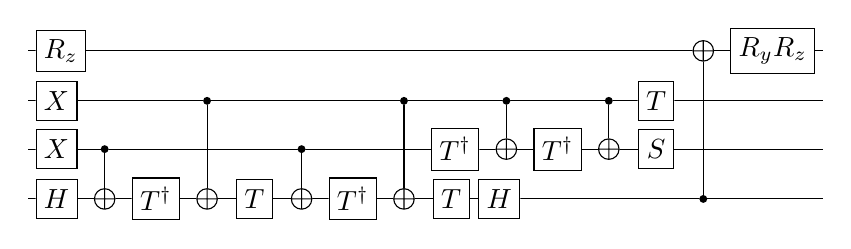
\begin{tikzpicture}[baseline=(current bounding box.center)]
                    \begin{yquant}
                        qubit {} q[4];
                        x q[1,2];
                        h q[3];
                        not q[3] | q[2];
                        box {$T^\dag$} q[3];
                        not q[3] | q[1];
                        box {$T$} q[3];
                        not q[3] | q[2];
                        box {$T^\dag$} q[3];
                        not q[3] | q[1];
                        box {$T$} q[3];
                        h q[3];
                        box {$T^\dag$} q[2];
                        not q[2] | q[1];
                        box {$T^\dag$} q[2];
                        not q[2] | q[1];
                        box {$T$} q[1];
                        box {$S$} q[2];
                        box {$R_z$} q[0];
                        not q[0] | q[3];
                        box {$R_y R_z$} q[0];
                    \end{yquant}
                \end{tikzpicture}
                \cdots
            \end{equation*}
        \item In general, the size of the decomposed circuit is exponential in the number of qubits
    \end{itemize}
\end{frame}

\begin{frame}
    \frametitle{Lessons Learned}
    \begin{itemize}
        \item I knew decomposition to \textsc{cnot} and single-qubit gates was possible, but had to learn how
        \item I learned that decompositions of general unitary matrices grow exponentially in the number of qubits
        \item Qiskit has a more efficient and practical approach, where the definition of each gate includes a decomposition
    \end{itemize}
\end{frame}

\begin{frame}
    \frametitle{Potential Uses}
    \begin{itemize}
        \item Decomposition would be useful if it was not so inefficient
        \item Building a unitary matrix from a circuit could be useful, but other tools can already to it
        \item Likely most useful as an educational tool to understand the mapping between quantum circuits and unitary matrices
    \end{itemize}
\end{frame}

\begin{frame}
    \frametitle{References and Links}
    \begin{itemize}
        \item Decomposition based on Sections 4.2, 4.3 and 4.5 of: \\
            Nielsen, M.\ A., \& Chuang, I.\ L. (2010). \emph{Quantum Computation and Quantum Information} (10th Anniversary ed.). Cambridge University Press.
        \item Code available at: \\
            \url{https://github.com/ulrikdem/cse60932-project}
    \end{itemize}
\end{frame}

\end{document}
